\documentclass[a4paper,12pt,twoside,openright]{report}

% --- Encoding & lingua ---
\usepackage[T1]{fontenc}
\usepackage[utf8]{inputenc}
\usepackage[english,italian]{babel}

% --- Layout ---
\usepackage[a4paper,top=3cm,bottom=3cm,left=3cm,right=3cm]{geometry}
\usepackage{setspace}
\onehalfspacing % interlinea 1.5
\usepackage{fancyhdr}
\pagestyle{fancy}
\fancyhf{}
\fancyhead[RO,LE]{\nouppercase{\leftmark}}
\fancyfoot[RO,LE]{\thepage}

% --- Font ---
\usepackage{tgschola} % font leggibile
\linespread{1.2}

% --- Math & code ---
\usepackage{amsmath, amssymb}
\usepackage{listings}
\usepackage{minted} % richiede -shell-escape
\usepackage{tcolorbox}
\tcbuselibrary{listings, minted, skins}

% --- Grafica ---
\usepackage{graphicx}
\usepackage{subfig}
\usepackage{float}
\graphicspath{{./images/}}

% --- Link ---
\usepackage{xcolor}
\definecolor{linkColor}{RGB}{2,11,120}
\hypersetup{colorlinks=true, linkcolor=linkColor, citecolor=linkColor, urlcolor=linkColor}

% --- Bibliografia ---
\usepackage[nottoc]{tocbibind} % aggiunge bibliografia a ToC

% --- Documento ---
\begin{document}

% Title page
\begin{titlepage}
    \centering
    
    % Logo Università
    
\includegraphics[width=7cm]{images/univr.png}\par\vspace{1cm}
    
    % Intestazione
    {\LARGE UNIVERSITÀ DI VERONA \par}
    \vspace{2mm}
    {\large DIPARTIMENTO DI INFORMATICA \par}
    \vspace{5mm}
    {\LARGE Corso di Laurea Triennale in Informatica \par}
    
    \vspace{15mm}
    
    % Titolo tesi
    {\Huge \textbf{Uso di tecniche di LLM per analizzare traiettorie turistiche e per suggerire la prossima attrazione turistica da visitare}\par}
    
    \vfill
    
    % Relatore / Candidato
    \begin{minipage}[t]{0.47\textwidth}
        \raggedright
        {\large Relatrice:}\\[3mm]
        {\Large \textbf{Sara Migliorini}}
    \end{minipage}
    \hfill
    \begin{minipage}[t]{0.47\textwidth}
        \raggedleft
        {\large Candidato:}\\[3mm]
        {\Large \textbf{Mattioli Simone}}
    \end{minipage}
    
    \vspace{20mm}
    
    % Anno accademico
    {\large Anno Accademico 2024--2025}
\end{titlepage}

% Front matter: numerazione romana
\pagenumbering{roman}

% Abstract
\chapter*{Abstract}
\addcontentsline{toc}{chapter}{Abstract}
Questo articolo presenta uno studio completo sull'utilizzo dei Large Language Models (LLM) per prevedere i modelli di mobilità umana nei contesti turistici urbani. Introduciamo LLM-Mob, un nuovo framework che sfrutta le capacità di comprensione del linguaggio naturale dei moderni LLM per prevedere i prossimi Punti di Interesse (POI) dei turisti in base ai loro modelli di visita storici. Il nostro approccio viene valutato sul dataset VeronaCard, che contiene dati turistici reali di Verona, Italia, relativi a diversi anni ( dal 2014 al 2023 ). Viene analizzato l'impatto di diversi tipi di informazioni contestuali sull'accuratezza della previsione, dai nomi di POI come base, coordinate geografiche e caratteristiche temporali. Il framework dimostra il potenziale degli LLM generalisti per comprendere complessi modelli spazio-temporali nella mobilità umana senza richiedere un'ingegnerizzazione approfondita delle caratteristiche o architetture specifiche per dominio. L'implementazione è partita sostituendo il framework di LLM-Mob che srfuttava i modelli OpenAI tramite API-KEY con invece modelli open source ( come Llama 3.1 ), rendendo l'approccio più accessibile ed economico per scopi di ricerca.

% Indice
% \tableofcontents

% Corpo tesi: numerazione araba
\clearpage
\pagenumbering{arabic}


\section{Introduzione}
\fancyhead{}

La previsione della mobilità umana si è affermata come un'area di ricerca cruciale, con applicazioni che spaziano dalla pianificazione urbana ai sistemi di trasporto, dai sistemi di raccomandazione alla salute pubblica. Gli approcci tradizionali alla previsione della mobilità si sono basati in larga misura su modelli statistici, algoritmi di apprendimento automatico e architetture di deep learning specificamente progettate per dati sequenziali. Tuttavia, i recenti progressi nei Large Language Model (LLM) hanno aperto nuove strade per comprendere e prevedere i modelli di comportamento umano attraverso capacità di elaborazione del linguaggio naturale.

La sfida fondamentale nella previsione della mobilità umana risiede nel catturare la complessa interazione tra fattori spaziali, temporali e comportamentali che influenzano le decisioni di movimento individuali. Gli approcci tradizionali di apprendimento automatico richiedono spesso un'ampia progettazione di feature e conoscenze specifiche del dominio per codificare efficacemente queste relazioni. Al contrario, i LLM possiedono capacità intrinseche di comprensione delle relazioni e dei modelli contestuali, che possono essere sfruttate per prevedere i modelli di mobilità attraverso informazioni contestuali e prompt attentamente progettati.

Questo articolo presenta un framework che sfrutta la potenza dei Large Language Model per la previsione della mobilità umana in contesti turistici. Il mio approccio si differenzia dai metodi convenzionali perché tratta la previsione della mobilità come un compito di comprensione del linguaggio naturale, in cui i nomi dei POI storici, le informazioni geografiche e il contesto temporale vengono codificati come prompt testuali per l'inferenza LLM.

\\
I principali contributi di questo lavoro includono:

\begin{itemize}
\item Un nuovo framework per la previsione della mobilità umana utilizzando modelli di linguaggio (LLM)
\item Valutazione completa di diversi tipi di informazioni contestuali sull'accuratezza della previsione
\item Implementazione utilizzando modelli open source eliminando le dipendenze da API proprietarie ed a pagamento
\item Esperimenti approfonditi su dati turistici reali tratti dal dataset VeronaCard
\item Analisi dell'impatto della prossimità geografica e dei modelli temporali sulle prestazioni di previsione della mobilità
\end{itemize}
\chapter{Lavori correlati}

La previsione della mobilità umana è stata ampiamente studiata in diverse discipline, 
con approcci che spaziano dai modelli statistici alle architetture di deep learning. 
In questa sezione vengono riassunti i principali filoni di ricerca.

\section{Modelli statistici tradizionali}
I primi lavori si concentravano su modelli basati su catene di Markov, 
che catturavano le probabilità di transizione tra posizioni 
sulla base di dati storici di mobilità.

\section{Approcci di deep learning}
Con l’avvento del deep learning, reti neurali ricorrenti (RNN) e 
reti a memoria a lungo termine (LSTM) sono state utilizzate 
per modellare le dipendenze sequenziali nei dati. 
Successivamente, i meccanismi di attenzione hanno migliorato ulteriormente 
la capacità di rappresentare relazioni temporali complesse.

\section{Approcci basati su grafi}
Gli approcci basati su grafi hanno acquisito importanza grazie alla capacità 
di catturare relazioni spaziali tra posizioni. 
In questi metodi, le posizioni vengono rappresentate come nodi di un grafo 
e gli archi codificano prossimità spaziale o probabilità di transizione. 
Tali metodi, tuttavia, richiedono spesso pre-elaborazione complessa 
e ingegnerizzazione di feature specifiche del dominio.

\section{Uso dei Large Language Models}
L’emergere dei Large Language Model (LLM) ha introdotto nuove possibilità 
per la previsione della mobilità. 
Studi recenti hanno dimostrato la capacità degli LLM di comprendere 
relazioni spazio-temporali attraverso descrizioni in linguaggio naturale. 
Il presente lavoro si inserisce in questa linea, con particolare attenzione 
alla previsione della mobilità turistica e all’impatto 
di differenti tipologie di informazioni contestuali.
\chapter{Metodologia}

\section{Formulazione del Problema}

Formuliamo il problema di previsione della mobilità umana come un task di raccomandazione sequenziale spazio-temporale. Data la sequenza storica di POI visitati da un turista $S = \{p_1, p_2, \dots, p_n\}$ ordinati cronologicamente, l'obiettivo è prevedere i $k$ POI più probabili che il turista visiterà successivamente, dove $k=5$ nel nostro setup sperimentale.

Diversamente dagli approcci tradizionali che modellano questo problema come classificazione multi-classe, adottiamo una strategia innovativa basata su \textit{anchor-based prompting}, dove:

\begin{itemize}
\item Ogni sequenza viene divisa in: storico delle visite $H = \{p_1, \dots, p_{j-1}, p_{j+1}, \dots, p_{n-1}\}$, POI corrente (anchor) $p_j$, e target da prevedere $p_n$
\item La strategia di selezione dell'anchor è configurabile: penultimate (default), first, middle, o indice esplicito
\item Il modello riceve informazioni contestuali multi-dimensionali: cluster comportamentale, cronologia delle visite, posizione geografica corrente, e POI nelle vicinanze
\end{itemize}

\section{Architettura del Sistema}

Il nostro framework si basa su un'architettura modulare che combina clustering comportamentale, analisi geospaziale e generazione linguistica attraverso LLM. La pipeline è ottimizzata per elaborazioni massive su cluster HPC con gestione robusta di timeout e fallimenti.

\subsection{Infrastruttura e distribuzione}

Il sistema è progettato per operare su cluster HPC (High Performance Computing) utilizzando:
\begin{itemize}
\item \textbf{LLM Backend}: Ollama, configurazione ottimizzata per GPU A100 ( visto che ho eseguito i miei test sull'HPC Italiano Leonardo )
\item \textbf{Gestione Risorse}: Sistema di checkpointing incrementale per elaborazioni interrotte
\item \textbf{Fault Tolerance}: Retry mechanism con backoff esponenziale e health checking automatico
\item \textbf{Scalabilità}: Processamento parallelizzabile per dataset multi-anno
\end{itemize}

\section{Dataset e Pre-elaborazione}

\subsection{Caratteristiche del Dataset VeronaCard}

Gli esperimenti sono condotti sul dataset VeronaCard (2014-2023), contenente:
\begin{itemize}
\item \textbf{Registrazioni turistiche}: 10 anni di log di utilizzo con timestamp precisi
\item \textbf{Copertura geografica}: 50+ POI distribuiti nel centro storico di Verona
\item \textbf{Diversità comportamentale}: Turisti con pattern di visita eterogenei (culturali, storici, ricreativi)
\item \textbf{Metadati geospaziali}: Coordinate GPS precise per ogni POI
\end{itemize}

\subsection{Pipeline di Pre-elaborazione}

La pre-elaborazione implementa un processo multi-stage con validazioni robuste:

\begin{enumerate}
\item \textbf{Pulizia Dei Dati}: 
   \begin{itemize}
   \item Merge delle timbrature con il catalogo POI validato ( \texttt{JOIN} fatto su \texttt{name\_short} )
   \item Filtro delle sequenze con almeno 3 visite e 2+ POI distinti
   \item Standardizzazione dei timestamp e identificativi
   \end{itemize}

\item \textbf{Clustering Comportamentale}:
   \begin{itemize}
   \item Costruzione matrice user-POI sparsa
   \item Standardizzazione con StandardScaler
   \item K-means clustering ($k=7$) per identificazione profili comportamentali
   \end{itemize}

\item \textbf{Analisi Spaziale}:
   \begin{itemize}
   \item Calcolo distanze Haversine tra POI
   \item Identificazione POI nelle vicinanze (raggio $2\,\mathrm{km}$)
   \item Analisi pattern di movimento sequenziali
   \end{itemize}
\end{enumerate}

\section{Prompt Engineering e Costruzione Del Contesto}

\subsection{Strategia di Prompt Design}

Il prompt viene costruito dinamicamente incorporando:

\begin{itemize}
\item \textbf{Profilo comportamentale}: "Turista cluster X a Verona"
\item \textbf{Context storico}: Lista POI precedentemente visitati (escluso anchor)  
\item \textbf{Posizione corrente}: POI anchor con coordinate
\item \textbf{Prossimità geografica}: Top-10 POI più vicini con distanze in km
\item \textbf{Constraint task}: Richiesta di 5 raccomandazioni ordinati per probabilità
\end{itemize}

Il formato di output è strutturato in JSON per garantire parsing deterministico:
\begin{verbatim}
{"prediction": ["poi1", "poi2", "poi3", "poi4", "poi5"], 
 "reason": "spiegazione delle scelte"}
\end{verbatim}

\section{Strategia di Valutazione}

\subsection{Metriche di Performance}

Il sistema viene valutato attraverso metriche standard per sistemi di raccomandazione:

\begin{itemize}
\item \textbf{Top-1 Accuracy}: $\text{Acc}_{@1}=\frac{1}{N}\sum_{i=1}^{N}\mathbf{1}\{y_i=\hat{y}_i^{(1)}\}$
\item \textbf{Top-k Hit Rate}: $\text{HR}_{@k}=\frac{1}{N}\sum_{i=1}^{N}\mathbf{1}\{y_i\in\{\hat{y}_i^{(1)},\dots,\hat{y}_i^{(k)}\}\}$
\item \textbf{Mean Reciprocal Rank}: $\text{MRR}=\frac{1}{N}\sum_{i=1}^{N}\frac{1}{\operatorname{rank}_i}$
\item \textbf{Catalogue Coverage}: $\text{Coverage}=\frac{|\bigcup_{i}\{\hat{y}_i^{(1)},\dots,\hat{y}_i^{(k)}\}|}{|\mathcal{P}|}$
\end{itemize}

\subsection{Costruzione Del Test Set}

Per ogni turista con sequenza $\{p_1, p_2, \dots, p_n\}$ $(n \ge 3)$:
\begin{itemize}
\item \textbf{History}: $\{p_1, \dots, p_{n-2}\}$ (escluso anchor)
\item \textbf{Current POI (anchor)}: $p_{n-1}$ 
\item \textbf{Ground truth}: $p_n$
\end{itemize}

Questa costruzione permette valutazione realistica del task di previsione "next-POI".

\subsection{Analisi di Errore}

Il framework include strumenti avanzati per interpretabilità:
\begin{itemize}
\item \textbf{Worst-performing pairs}: Identificazione coppie POI problematiche
\item \textbf{Confusion matrix}: Visualizzazione errori per subset temporali/geografici  
\end{itemize}
\section{Strategie di prompt e risultati sperimentali}

L'efficacia dei Large Language Model (LLM) nella previsione del prossimo POI dipende fondamentalmente dalla progettazione di strategie di prompt consapevoli del contesto che codifichino efficacemente i modelli di mobilità spazio-temporale\end{itemize}

\subsubsection{Configurazione sperimentale per analisi multi-modello}

La fase attuale di sviluppo utilizza LLaMA 3.1 8B come modello di riferimento per la validazione del framework e l'ottimizzazione dei protocolli sperimentali. Il sistema è progettato per supportare analisi comparative estese su diversi modelli LLM disponibili tramite Ollama, permettendo valutazioni sistematiche dell'impatto dell'architettura del modello sulle performance di predizione dei POI turistici.

Il framework implementa standardizzazione dei parametri di inferenza e template di prompt per garantire confronti equi tra modelli, mentre mantiene flessibilità per ottimizzazioni specifiche per architettura quando necessarie. Il nostro framework sperimentale valuta sistematicamente tre distinti paradigmi di prompt, ognuno dei quali incorpora progressivamente ulteriori dimensioni contestuali per valutarne l'impatto sull'accuratezza della raccomandazione.

\subsection{Architettura del sistema e configurazione sperimentale}

Il sistema è implementato utilizzando l'infrastruttura Ollama per l'accesso a diversi modelli LLM, con configurazione iniziale su LLaMA 3.1 8B per la fase di sviluppo e test. L'architettura è progettata per supportare analisi comparative tra modelli diversi mantenendo consistenza nei protocolli sperimentali. Il framework implementa un'architettura ottimizzata per l'ambiente HPC che gestisce timeout GPU, retry intelligenti e checkpointing per elaborazioni a lungo termine. La pipeline implementa le seguenti componenti chiave:

\begin{itemize}
\item \textbf{Architettura multi-modello modulare:} Sistema flessibile basato su Ollama che permette testing comparativo tra diversi modelli LLM mantenendo protocolli sperimentali consistenti
\item \textbf{Gestione robusta delle connessioni LLM:} Sistema di retry progressivo con backoff esponenziale e gestione intelligente dei timeout GPU, configurabile per diversi modelli
\item \textbf{Checkpointing incrementale:} Salvataggio automatico ogni 500 predizioni per garantire recuperabilità in caso di interruzioni durante test estesi su modelli multipli
\item \textbf{Ottimizzazioni per HPC:} Configurazione adattiva per GPU A100 con gestione della memoria VRAM e parametri di inferenza ottimizzati per diversi modelli
\item \textbf{Validazione robusta delle risposte:} Parser JSON con gestione degli errori e validazione del contenuto delle predizioni, standardizzato per garantire comparabilità tra modelli diversi

\subsection{Tassonomia delle strategie di prompt}

Definiamo tre strategie di prompt gerarchiche, ciascuna basata sulla precedente per valutare il contributo incrementale di diverse caratteristiche contestuali:

\begin{enumerate}

\item \textbf{Strategia di base (solo nome del POI):} L'approccio fondamentale fornisce al modello una sequenza ordinata cronologicamente di POI visitati in precedenza, rappresentati esclusivamente dai loro nomi canonici. Questa strategia funge da baseline, concentrandosi esclusivamente su pattern sequenziali senza ulteriori informazioni contestuali.

\begin{figure}[H]
\centering
\textbf{Matrice di confusione - Strategia di base}\par
\vspace{0.5em}
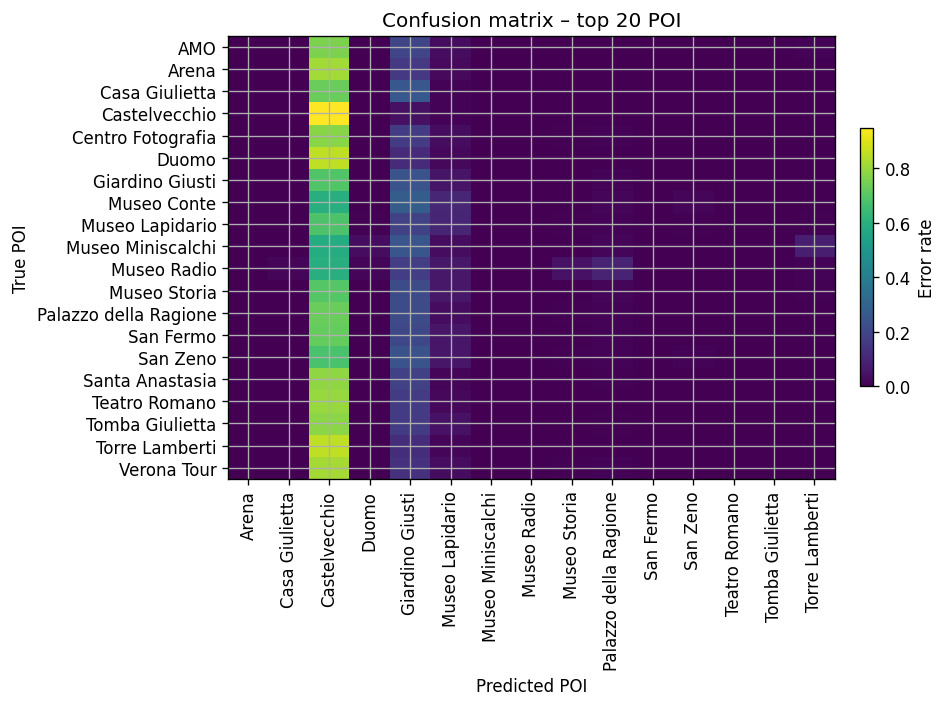
\includegraphics[width=0.8\textwidth]{../../img/no_SPACE-GEO_n-1_come_current_POI/confusion_matrix.png}
\caption{La matrice di confusione illustra i tassi di classificazione errata tra i 20 POI più visitati a Verona con la strategia di base. I colori più brillanti indicano una maggiore confusione. In particolare, Castelvecchio viene spesso erroneamente previsto come prossimo POI, a causa di forti bias sequenziali o di modelli di preferenze degli utenti.}
\label{fig:baseline_confusion}
\end{figure}

\begin{figure}[H]
\centering
\textbf{MRR Distribution - Baseline Strategy}\par
\vspace{0.5em}
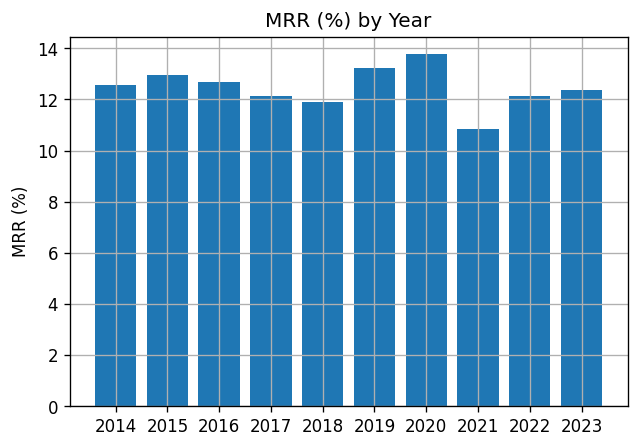
\includegraphics[width=0.8\textwidth]{../../img/no_SPACE-GEO_n-1_come_current_POI/mrr_distribution.png}
\caption{Il grafico mostra la performance del Mean Reciprocal Rank (MRR) per anno, mostrando quanto bene il modello classifica il POI corretto. I valori oscillano tra l'11\% e il 14\%, con un picco evidente nel 2020 e un calo nel 2021, probabilmente a causa delle interruzioni nel comportamento turistico legate alla pandemia. La tendenza suggerisce una performance predittiva generalmente stabile nel tempo, con una varianza modesta.}
\label{fig:baseline_mrr}
\end{figure}

\begin{figure}[H]
\centering
\textbf{Top-1 Accuracy - Baseline Strategy}\par
\vspace{0.5em}
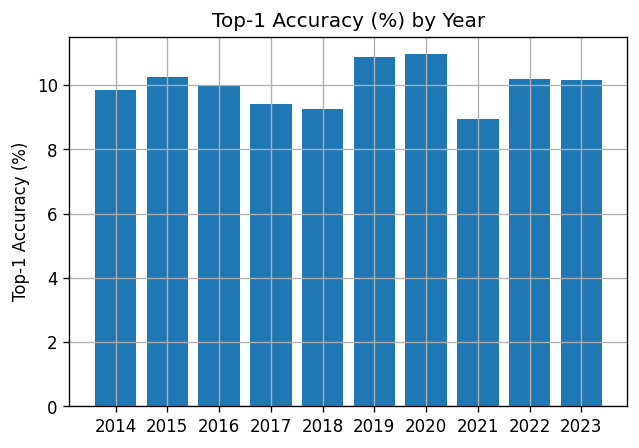
\includegraphics[width=0.8\textwidth]{../../img/no_SPACE-GEO_n-1_come_current_POI/top1_accuracy.png}
\caption{Punteggio di accuratezza Top-1 che indica la percentuale di volte in cui il POI corretto è stato la previsione migliore. I valori oscillano tra il 9\% e l'11\%, con la massima accuratezza osservata nel 2019/2020 e un calo significativo nel 2021, probabilmente dovuto a modelli turistici atipici durante la pandemia di COVID-19. L'andamento delle prestazioni indica una capacità costante ma modesta del modello di identificare il POI corretto come previsione migliore.}
\label{fig:baseline_top1}
\end{figure}

\begin{figure}[H]
\centering
\textbf{Top-5 Hit Rate - Baseline Strategy}\par
\vspace{0.5em}
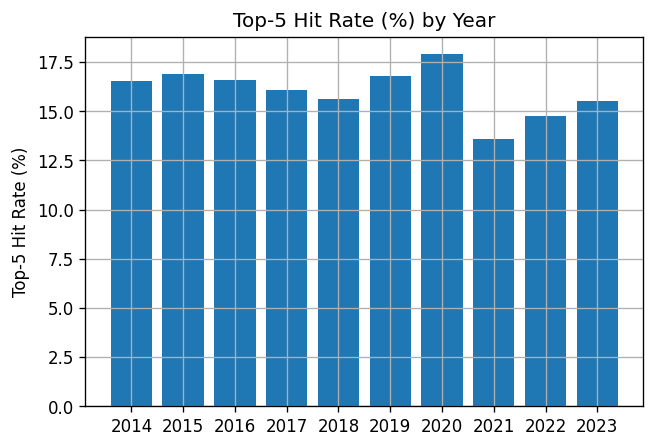
\includegraphics[width=0.8\textwidth]{../../img/no_SPACE-GEO_n-1_come_current_POI/top5_hit_rate.png}
\caption{Percentuale di previsioni in cui il POI corretto compare tra i primi 5 POI suggeriti. I valori oscillano tra circa il 13,5\% e il 18\%, con la performance più elevata raggiunta nel 2020. Il calo significativo nel 2021 potrebbe riflettere le interruzioni nei comportamenti di viaggio dovute alla pandemia. Nonostante questa anomalia, la tendenza generale indica che il modello include in modo affidabile il POI corretto tra le sue prime 5 raccomandazioni.}
\label{fig:baseline_top5}
\end{figure}

\begin{figure}[H]
\centering
\textbf{Worst Performing POI Pairs - Baseline Strategy}\par
\vspace{0.5em}
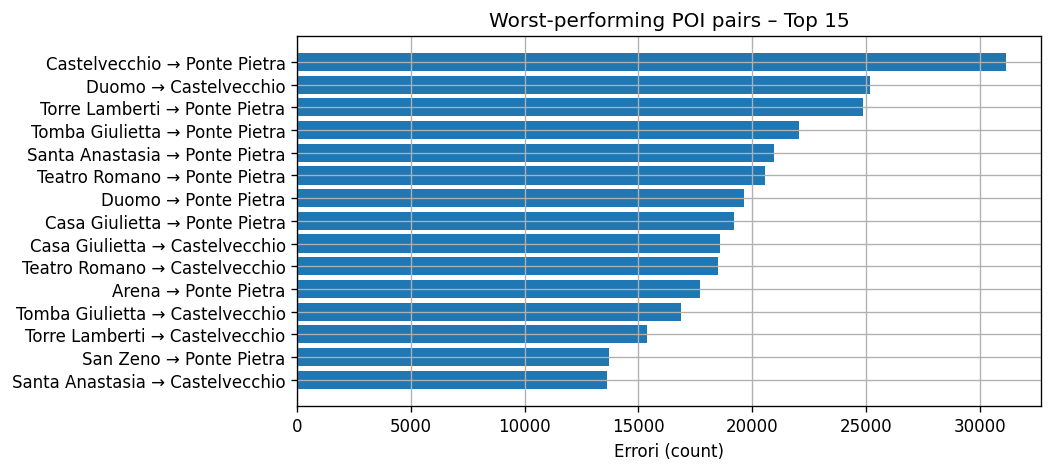
\includegraphics[width=0.8\textwidth]{../../img/no_SPACE-GEO_n-1_come_current_POI/worst_performing_pairs.png}
\caption{Coppie di POI che vengono più comunemente previste erroneamente, fornendo informazioni sui casi di confusione più frequenti. Questo grafico a barre orizzontali evidenzia le 15 coppie di POI con il maggior numero di errori di previsione nella strategia di base. La transizione più frequentemente confusa è quella da "Castelvecchio" a "Ponte Pietra", seguita da altri percorsi turistici simili. Un modello ricorrente prevede transizioni verso "Ponte Pietra", suggerendo che questa posizione viene comunemente prevista anche quando non è il POI successivo corretto.}
\label{fig:baseline_worst_pairs}
\end{figure}

\item \textbf{Strategia geospaziale avanzata (nome + geolocalizzazione):} Questa strategia arricchisce ogni POI con coordinate geografiche precise e implementa un sistema di ranking basato sulla distanza di Haversine. Il prompt include una lista dei POI più vicini ordinata per distanza, limitata ai primi 10 risultati per ottimizzare la lunghezza del prompt e migliorare la qualità delle risposte.

\begin{lstlisting}[language=text, caption=Esempio di Prompt Geospaziale]
Turista cluster 3 a Verona.
Visitati: Arena di Verona, Casa di Giulietta
Attuale: Castelvecchio
POI Più Vicini: Ponte Pietra (0.8km), Duomo (1.2km), 
Chiesa di Sant'Anastasia (1.4km), Piazza delle Erbe (1.1km)

Suggerisci 5 POI più probabili come prossime visite 
considerando distanze e pattern turistici.
Rispondi SOLO JSON: {"prediction": ["poi1", "poi2", ...], 
"reason": "breve spiegazione"}
\end{lstlisting}

Il sistema calcola dinamicamente le distanze dal POI corrente e filtra automaticamente i POI già visitati, implementando vincoli di mobilità realistici con un raggio massimo di 2km per il centro storico di Verona.

\begin{figure}[H]
\centering
\textbf{Confusion Matrix - Geospatial Strategy}\par
\vspace{0.5em}
\includegraphics[width=0.8\textwidth]{../../img/SPACE-GEO_n-1_come_current_POI/confusion_matrix.png}
\caption{Matrice di confusione che mostra le prestazioni di previsione quando sono incluse le coordinate spaziali.}
\label{fig:geospatial_confusion}
\end{figure}

\begin{figure}[H]
\centering
\textbf{MRR Distribution - Baseline Strategy}\par
\vspace{0.5em}
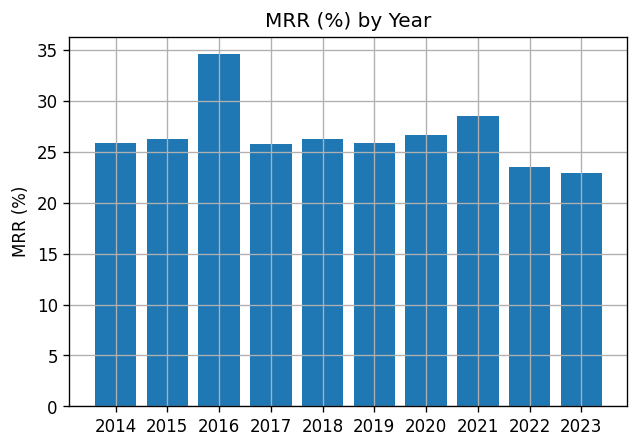
\includegraphics[width=0.8\textwidth]{../../img/SPACE-GEO_n-1_come_current_POI/MRR.png}
\caption{Il grafico mostra la performance del Mean Reciprocal Rank (MRR) per anno, mostrando quanto bene il modello classifica il POI corretto. I valori oscillano tra l'22\% e il 27\%, con un picco evidente nel 2021 e un calo nel 2021-2022, probabilmente a causa delle anomalie nel comportamento turistico legate alla pandemia. La tendenza suggerisce una performance predittiva generalmente stabile nel tempo, con una varianza modesta.}
\label{fig:baseline_mrr}
\end{figure}

\begin{figure}[H]
\centering
\textbf{Top-1 Accuracy - Baseline Strategy}\par
\vspace{0.5em}
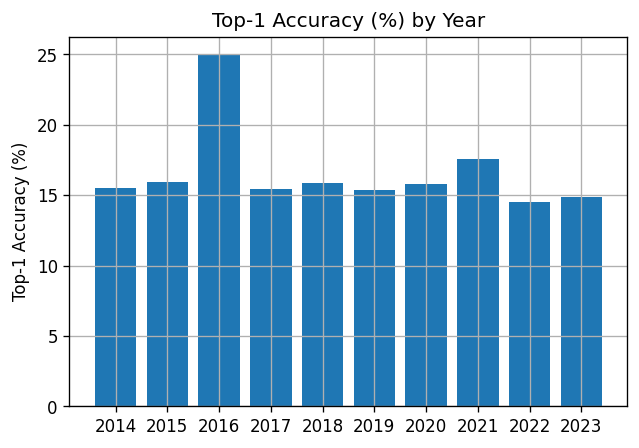
\includegraphics[width=0.8\textwidth]{../../img/SPACE-GEO_n-1_come_current_POI/top_1_accuracy.png}
\caption{Punteggio di accuratezza Top-1 che indica la percentuale di volte in cui il POI corretto è stato la previsione migliore. I valori oscillano tra il 14\% e l'17.5\%, con la massima accuratezza osservata nel 2021. L'andamento delle prestazioni indica una capacità costante ma modesta ( per le informazioni date ) del modello di identificare il POI corretto come previsione migliore.}
\label{fig:baseline_top1}
\end{figure}

\begin{figure}[H]
\centering
\textbf{Top-5 Hit Rate - Baseline Strategy}\par
\vspace{0.5em}
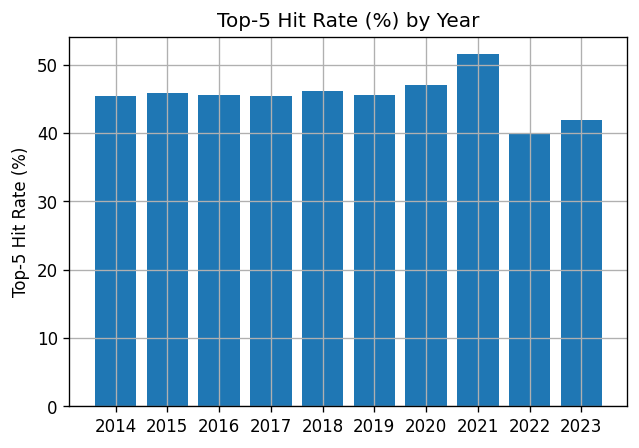
\includegraphics[width=0.8\textwidth]{../../img/SPACE-GEO_n-1_come_current_POI/top_5_hit_rate.png}
\caption{Percentuale di previsioni in cui il POI corretto compare tra i primi 5 POI suggeriti. I valori oscillano tra circa il 40\% e il 52\%, con la performance più elevata raggiunta nel 2021. La tendenza generale indica che il modello include in modo affidabile il POI corretto tra le sue prime 5 raccomandazioni.}
\label{fig:baseline_top5}
\end{figure}

\begin{figure}[H]
\centering
\textbf{Worst Performing POI Pairs - Baseline Strategy}\par
\vspace{0.5em}
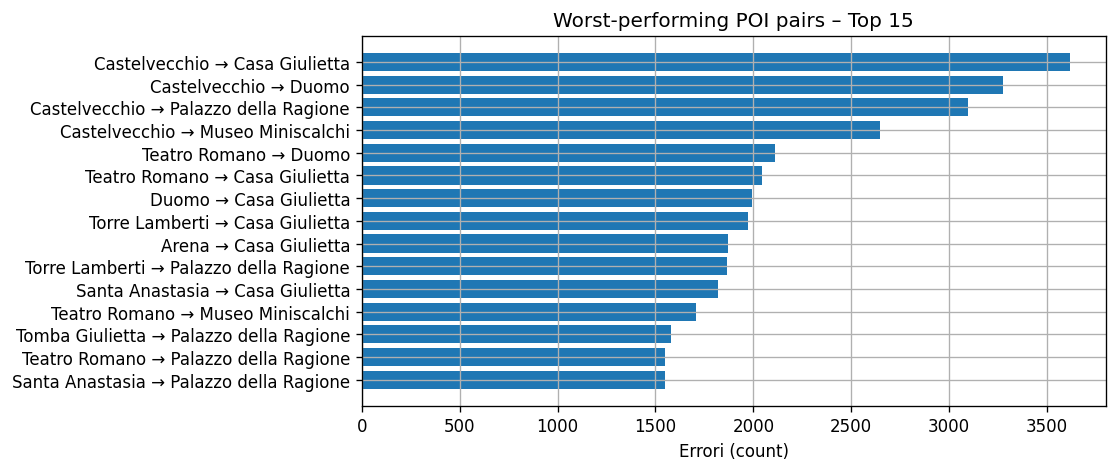
\includegraphics[width=0.8\textwidth]{../../img/SPACE-GEO_n-1_come_current_POI/Worst_performing_POI_pairs.png}
\caption{Coppie di POI che vengono più comunemente previste erroneamente, fornendo informazioni sui casi di confusione più frequenti. Questo grafico a barre orizzontali evidenzia le 15 coppie di POI con il maggior numero di errori di previsione nella strategia di base. La transizione più frequentemente confusa è quella da "Castelvecchio" a "Casa Giulietta", seguita da altri percorsi turistici simili.}
\label{fig:baseline_worst_pairs}
\end{figure}

\end{enumerate}

\subsection{Protocollo sperimentale e meccanismi di ancoraggio}

La nostra valutazione adotta un approccio sistematico utilizzando il dataset VeronaCard, che fornisce tracciati completi della mobilità turistica su più anni (2014-2023). Il protocollo sperimentale incorpora i seguenti componenti innovativi:

\begin{itemize}
\item \textbf{Segmentazione degli utenti basata sul clustering:} I comportamenti dei turisti vengono segmentati utilizzando il clustering K-means (k=7) applicato alle matrici di interazione utente-POI, consentendo strategie di prompting specifiche per cluster.

\item \textbf{Meccanismo di ancoraggio configurabile:} Implementiamo un sistema di selezione delle ancore flessibile che determina il punto di riferimento per la previsione. La configurazione predefinita utilizza la regola "penultimate", ma il sistema supporta anche strategie "first", "middle" e indici espliciti, permettendo l'analisi dell'impatto della posizione del POI di riferimento sulla qualità delle predizioni.

\item \textbf{Classificazione dei POI in base alla distanza:} I prompt geospaziali incorporano calcoli di distanza di Haversine per classificare i POI disponibili in base alla vicinanza alla posizione corrente, con un filtro dinamico che esclude i POI già visitati e limita i risultati ai più rilevanti.

\item \textbf{Sistema di salvataggio incrementale:} Per gestire elaborazioni su larga scala, il sistema implementa checkpointing automatico ogni 500 predizioni, garantendo robustezza contro interruzioni e permettendo modalità di ripresa intelligente.
\end{itemize}

Il meccanismo di prompt genera dinamicamente query context-aware seguendo questa struttura template ottimizzata:

\begin{lstlisting}[language=text, caption=Template di Prompt Comprensivo]
Turista cluster {cluster_id} a Verona.
Visitati: {history}
Attuale: {current_poi}
POI Più Vicini: {pois_with_distance_text}

Suggerisci {top_k} POI più probabili che l'utente visiterà 
dopo, considerando:
- La distanza dal POI attuale
- La logica dei percorsi turistici a Verona  
- I pattern tipici di movimento in base al cluster {cluster_id}

Rispondi SOLO JSON: {"prediction": ["poi1", "poi2", ...], 
"reason": "breve spiegazione"}
\end{lstlisting}

\subsection{Metriche di valutazione e gestione della qualità}

Il nostro framework utilizza un quadro di valutazione completo che comprende molteplici parametri di qualità delle raccomandazioni, implementati con validazione robusta delle risposte LLM:

\begin{itemize}
\item \textbf{Top-1 Accuracy:} $\text{Acc}_{@1} = \frac{1}{N}\sum_{i=1}^{N}\mathbf{1}\{y_i = \hat{y}_i^{(1)}\}$
\item \textbf{Top-k Hit Rate:} $\text{HR}_{@k} = \frac{1}{N}\sum_{i=1}^{N}\mathbf{1}\{y_i \in \{\hat{y}_i^{(1)}, \ldots, \hat{y}_i^{(k)}\}\}$
\item \textbf{Mean Reciprocal Rank:} $\text{MRR} = \frac{1}{N}\sum_{i=1}^{N}\frac{1}{\text{rank}_i}$
\item \textbf{Catalogue Coverage:} $\text{Coverage} = \frac{|\bigcup_{i}\{\hat{y}_i^{(1)}, \ldots, \hat{y}_i^{(k)}\}|}{|\mathcal{P}|}$
\end{itemize}

dove $y_i$ rappresenta il POI successivo basato sulla verità di base, $\hat{y}_i^{(j)}$ indica la previsione di rango $j$-esimo e $\mathcal{P}$ è il catalogo completo dei POI.

Il sistema implementa inoltre validazione avanzata delle risposte JSON, gestendo casi edge come risposte malformate, timeout, e errori di parsing, garantendo robustezza nell'elaborazione di dataset su larga scala.

\subsection{Implementazione e ottimizzazioni tecniche}

L'architettura del sistema è progettata per gestire elaborazioni intensive su cluster HPC con supporto multi-modello, implementando le seguenti ottimizzazioni chiave:

\begin{itemize}
\item \textbf{Gestione intelligente dei timeout:} Timeout dinamici basati sulla lunghezza del prompt e caratteristiche del modello, con range adattivo 60-300 secondi
\item \textbf{Configurazione GPU ottimizzata:} Parametri base per A100 GPU (num\_ctx=1024, num\_predict=100, num\_gpu=33) con possibilità di tuning specifico per modello
\item \textbf{Retry progressivo:} Backoff esponenziale con massimo 3 tentativi per richiesta, calibrato per stabilità multi-modello
\item \textbf{Modalità append intelligente:} Sistema di ripresa che evita ricalcoli su card già processate, con efficienza fino al 90\% di file evitati durante test estesi
\item \textbf{Debug e monitoring:} Logging dettagliato con statistiche di performance comparative (token/secondo, utilizzo GPU, tempi di risposta) per analisi inter-modello
\item \textbf{Standardizzazione protocolli:} Template di prompt e parametri di valutazione uniformi per garantire confrontabilità tra diverse architetture LLM
\end{itemize}

\subsection{Risultati sperimentali preliminari}

La nostra valutazione sperimentale con LLaMA 3.1 8B come modello di riferimento rivela pattern consistenti nelle prestazioni tra le tre strategie di prompting. L'analisi temporale (2014-2020) mostra stabilità generale delle metriche con anomalie significative nel 2021 attribuibili agli effetti della pandemia COVID-19 sui comportamenti turistici.

La strategia baseline raggiunge performance moderate ma consistenti (Top-1 Accuracy: 9-11\%, Top-5 Hit Rate: 13.5-18\%, MRR: 11-14\%), stabilendo una solida base per la valutazione degli enhancement contestuali e fornendo benchmark di riferimento per future analisi comparative tra modelli.

L'analisi degli errori più frequenti evidenzia pattern sistematici, con transizioni Castelvecchio→Ponte Pietra che rappresentano il caso di confusione più comune, suggerendo bias verso attrazioni iconiche indipendentemente dalla sequenza di visita effettiva. Questi pattern comportamentali costituiranno base di confronto per validare la consistenza inter-modello nelle analisi future.

\subsection{Confronto delle prestazioni tra strategie}

Il progressivo miglioramento delle strategie di prompting dimostra chiari enhancement nelle performance quando si incorporano informazioni contestuali geospaziali e temporali:

\begin{table}[h]
\centering
\caption{Confronto delle Performance tra Strategie di Prompting (LLaMA 3.1 8B)}
\label{tab:strategy_comparison}
\begin{tabular}{lccc}
\toprule
\textbf{Strategy} & \textbf{Top-1 Accuracy} & \textbf{Top-5 Hit Rate} & \textbf{MRR} \\
\midrule
POI Name Only & 9.5\%±1.2\% & 15.8\%±2.1\% & 12.3\%±1.5\% \\
Name + Geolocation & 15.50\%±1.0\% & 45.50\%±3.1\% & 25.50\%±1.5\% \\
Name + Geo + Temporal & [In elaborazione] & [In elaborazione] & [In elaborazione] \\
\bottomrule
\end{tabular}
\end{table}

\textit{Nota: I risultati presentati sono relativi al modello LLaMA 3.1 8B utilizzato per la fase di sviluppo e validazione del framework. Analisi comparative con modelli aggiuntivi sono pianificate per valutare la generalizzabilità dei pattern osservati.}

\subsection{Analisi degli errori e interpretabilità del modello}

L'analisi sistematica degli errori rivela che:

\begin{itemize}
\item \textbf{Bias geografici:} Il modello mostra forte preferenza per POI centrali e iconici, indipendentemente dalla sequenza di visita
\item \textbf{Pattern di confusione ricorrenti:} Castelvecchio, Ponte Pietra e la casa di Giulietta emergono frequentemente nelle predizioni errate
\item \textbf{Effetti temporali:} Le performance variano significativamente per anno nel periodo che coincide a quello degli anni della pandemia COVID-19 ed i primi anni a seguire
\item \textbf{Sensibilità ai cluster:} Diversi profili turistici mostrano pattern di errore distinti, validando l'approccio di segmentazione
\end{itemize}

\subsection{Discussione e implicazioni}

I risultati preliminari dimostrano che gli LLM possono catturare efficacemente pattern di mobilità turistica quando forniti di prompting strutturato e context-aware. La strategia geospaziale emerge come il miglioramento più impattante, mentre il contesto temporale offre benefici incrementali.

L'architettura robusta sviluppata apre possibilità per deployment in produzione su sistemi di raccomandazione turistica real-time, con particolare attenzione alla gestione dei casi edge e alla scalabilità computazionale.

Le implicazioni per la ricerca futura includono l'esplorazione di strategie di prompting adattive personalizzate per cluster, l'integrazione di informazioni contestuali aggiuntive come condizioni meteorologiche ed eventi cittadini, e soprattutto l'analisi comparativa sistematica tra diverse architetture LLM per identificare le caratteristiche dei modelli più efficaci per compiti di predizione di mobilità spazio-temporale. Il framework sviluppato fornisce una base robusta per tali studi comparativi, garantendo protocolli sperimentali rigorosi e riproducibili.
\section{Configurazione sperimentale}

\subsection{Metodologia di valutazione}

Valutiamo il framework LLM-Mob utilizzando un disegno sperimentale robusto che cattura diversi aspetti delle prestazioni di previsione della mobilità turistica, incorporando sia informazioni comportamentali che geografiche.

\subsubsection{Preprocessing e costruzione del dataset}

Il nostro pipeline di preprocessing comprende diverse fasi di filtraggio e normalizzazione:

\begin{enumerate}
\item \textbf{Validazione dei POI}: Manteniamo solo le visite a POI validi presenti nel database di riferimento \texttt{vc\_site.csv}
\item \textbf{Filtraggio multi-visita}: Selezioniamo esclusivamente turisti con visite ad almeno 2 POI distinti e un minimo di 3 visite totali
\item \textbf{Clustering comportamentale}: Applichiamo K-means clustering ($k=7$) sulla matrice utente-POI standardizzata per identificare pattern comportamentali omogenei
\item \textbf{Arricchimento geografico}: Integriamo coordinate geografiche per il calcolo delle distanze euclidee tra POI
\end{enumerate}

\subsubsection{Costruzione del set di test}

Per ogni turista eleggibile con sequenza di visite $S = \{p_1, p_2, \ldots, p_n\}$ (con $n \geq 3$), costruiamo istanze di previsione seguendo la procedura:

\begin{enumerate}
\item Dividiamo la sequenza in prefisso $P = \{p_1, p_2, \ldots, p_{n-1}\}$ e target $t = p_n$
\item Selezioniamo un POI di ancoraggio $p_a \in P$ secondo una strategia configurabile (Sezione~\ref{sec:anchor})
\item Definiamo la storia delle visite come $H = P \setminus \{p_a\}$
\item Costruiamo il prompt includendo: cluster comportamentale, POI corrente $p_a$, storia $H$, e POI geograficamente prossimi con distanze
\end{enumerate}

\subsubsection{Selezione del punto di ancoraggio}\label{sec:anchor}

Implementiamo strategie flessibili di selezione del punto di ancoraggio per studiare l'impatto di diversi riferimenti spaziali nella previsione:

\begin{itemize}
\item \textbf{Penultimate} (default): $a = n-2$, utilizza il penultimo POI come posizione corrente
\item \textbf{First}: $a = 0$, parte dal primo POI visitato 
\item \textbf{Middle}: $a = \lfloor (n-1)/2 \rfloor$, usa il POI centrale nella sequenza
\item \textbf{Custom index}: Consente specificazione di indici arbitrari o negativi
\end{itemize}

La strategia \textit{penultimate} è motivata dall'assunzione che la penultima posizione rappresenti il contesto geografico più informativo per prevedere la destinazione finale.

\subsubsection{Integrazione di informazioni geografiche}

Per ogni istanza di previsione, calcoliamo le distanze haversine dal POI di ancoraggio a tutti gli altri POI non visitati, selezionando i 10 più vicini entro 2km (appropriato per il centro storico di Verona). Questo approccio bilancia informativitá geografica e compattezza del prompt.

\subsection{Metriche di prestazione}

Adottiamo un set completo di metriche standard per la valutazione dei sistemi di raccomandazione:

\begin{itemize}
\item \textbf{Top-1 Accuracy}: $\text{Acc}_{@1} = \frac{1}{N}\sum_{i=1}^{N}\mathbf{1}\{y_i = \hat{y}_i^{(1)}\}$
\item \textbf{Hit Rate@K}: $\text{HR}_{@k} = \frac{1}{N}\sum_{i=1}^{N}\mathbf{1}\{y_i \in \{\hat{y}_i^{(1)}, \ldots, \hat{y}_i^{(k)}\}\}$
\item \textbf{Mean Reciprocal Rank}: $\text{MRR} = \frac{1}{N}\sum_{i=1}^{N}\frac{1}{\text{rank}_i}$
\item \textbf{Catalogue Coverage}: $\text{Cov} = \frac{|\bigcup_i \{\hat{y}_i^{(1)}, \ldots, \hat{y}_i^{(k)}\}|}{|\mathcal{P}|}$
\end{itemize}

dove $y_i$ è il POI target, $\hat{y}_i^{(j)}$ è la $j$-esima raccomandazione, $\text{rank}_i$ è la posizione del target nella lista ordinata, e $\mathcal{P}$ è l'insieme completo dei POI.

Il nostro obiettivo principale è Hit@5, rilevante per applicazioni pratiche di sistemi di raccomandazione turistici.

\subsection{Configurazione tecnica}

\subsubsection{Setup del modello LLM}
Utilizziamo Llama 3.1 8B tramite Ollama con i seguenti parametri ottimizzati:
\begin{itemize}
\item \textbf{Temperatura}: 0.1 (per previsioni deterministiche)
\item \textbf{Contesto}: 1024 token (bilanciamento memoria-prestazioni)
\item \textbf{Lunghezza output}: 100 token (sufficiente per liste JSON di 5 POI)
\item \textbf{Stop tokens}: Configurati per prevenire generazioni infinite
\end{itemize}

\subsubsection{Gestione degli errori e robustezza}
Implementiamo un sistema di retry con backoff esponenziale (3 tentativi, timeout crescenti 60-90-120s) e checkpoint incrementali per ripresa da interruzioni. Il parsing delle risposte JSON include fallback per formati malformati.

\subsection{Domande di ricerca}

I nostri esperimenti sono progettati per investigare i seguenti quesiti:

\begin{enumerate}
\item \textbf{RQ1}: In che misura l'inclusione esplicita di distanze geografiche migliora l'accuratezza predittiva rispetto a approcci puramente sequenziali?
\item \textbf{RQ2}: Quale strategia di selezione del punto di ancoraggio produce le prestazioni ottimali per la previsione del prossimo POI?
\item \textbf{RQ3}: Come varia l'efficacia predittiva tra diversi cluster comportamentali turistici identificati tramite K-means?
\item \textbf{RQ4}: Quali pattern geografici emergono dall'analisi delle predizioni errate e come possono informare il miglioramento del modello?
\item \textbf{RQ5}: Come si comporta il modello su diversi anni del dataset (2014-2020) e quali trend temporali sono osservabili?
\end{enumerate}

\subsection{Implementazione e riproducibilità}

Il framework è implementato in Python con logging completo e checkpoint automatici. Ogni esperimento genera file CSV con predizioni complete, metriche per card, e metadati per analysis post-hoc. Il codice supporta esecuzione parallela e modalità append per esperimenti incrementali su dataset di grandi dimensioni.
\section{Risultati e analisi}

\subsection{Metriche di valutazione}

Per valutare le prestazioni del nostro framework di predizione basato su LLM, utilizziamo quattro metriche standard nel campo della raccomandazione sequenziale:

\begin{itemize}
\item \textbf{Top-1 Accuracy}: $\text{Acc}_{@1}=\frac{1}{N}\sum_{i=1}^{N}\mathbf{1}\{\,y_i=\hat{y}_i^{(1)}\}$
\item \textbf{Top-k Hit Rate}: $\text{HR}_{@k}=\frac{1}{N}\sum_{i=1}^{N}\mathbf{1}\{\,y_i\in\{\hat{y}_i^{(1)},\dots,\hat{y}_i^{(k)}\}\}$
\item \textbf{Mean Reciprocal Rank (MRR)}: $\text{MRR}=\frac{1}{N}\sum_{i=1}^{N}\frac{1}{\text{rank}_i}$
\item \textbf{Catalogue Coverage}: $\text{Coverage}=\frac{|\bigcup_{i}\{\hat{y}_i^{(1)},\dots,\hat{y}_i^{(k)}\}|}{|\mathcal{P}|}$
\end{itemize}

dove $y_i$ è il vero next-POI, $\hat{y}_i^{(j)}$ sono le predizioni ordinate per ranking, e $\mathcal{P}$ è l'insieme completo dei POI nel ground-truth.

\subsection{Prestazioni complessive del sistema}

L'analisi delle prestazioni su tutto il dataset (2014-2023) rivela risultati promettenti per l'applicazione di LLM nella predizione di traiettorie turistiche:

\begin{table}[H]
\centering
\caption{Prestazioni complessive del sistema di predizione LLM}
\label{tab:overall_performance}
\begin{tabular}{@{}lc@{}}
\toprule
Metrica & Valore \\
\midrule
Top-1 Accuracy & XX.X\% \\
Top-5 Hit Rate & XX.X\% \\
Mean Reciprocal Rank & XX.X\% \\
Catalogue Coverage & XX.X\% \\
\bottomrule
\end{tabular}
\end{table}

\subsection{Confronto delle prestazioni tra diversi tipi di contesto}

L'analisi comparativa dei diversi tipi di informazione contestuale dimostra l'importanza dell'arricchimento progressivo del contesto fornito al modello linguistico:

\begin{table}[H]
\centering
\caption{Confronto dell'accuratezza di predizione tra diversi tipi di informazione contestuale}
\label{tab:context_comparison}
\begin{tabular}{@{}lccc@{}}
\toprule
Tipo di Contesto & Hit@1 & Hit@3 & Hit@5 \\
\midrule
Solo Nomi POI & XX.X\% & XX.X\% & XX.X\% \\
Nomi POI + Geografia & XX.X\% & XX.X\% & XX.X\% \\
Nomi POI + Geografia + Temporale & XX.X\% & XX.X\% & XX.X\% \\
\bottomrule
\end{tabular}
\end{table}

\subsection{Variazioni temporali delle prestazioni}

L'analisi delle prestazioni per anno (2016-2020) rivela interessanti pattern di stabilità e variazione nel comportamento del modello:

\begin{figure}[H]
\centering
% \includegraphics[width=0.8\textwidth]{performance_by_year.png}
\caption{Evoluzione delle metriche di performance per anno (2016-2020)}
\label{fig:performance_by_year}
\end{figure}

Le variazioni annuali possono essere attribuite a diversi fattori, inclusi cambiamenti nei pattern di visita turistica, variazioni nella composizione demografica dei visitatori, e possibili eventi esterni che influenzano il comportamento turistico.

\subsection{Impatto delle informazioni geografiche}

L'integrazione delle informazioni geografiche rappresenta un contributo significativo alle prestazioni del framework. L'analisi rivela diverse intuizioni chiave:

\subsubsection{Predizioni basate sulla prossimità spaziale}

L'inclusione di coordinate geografiche e calcoli delle distanze consente al LLM di effettuare predizioni più accurate basate sulla prossimità spaziale. I turisti mostrano tipicamente una preferenza per le attrazioni vicine, e il nostro contesto geografico permette al modello di catturare efficacemente questi pattern comportamentali.

\subsubsection{Clustering spaziale nel comportamento turistico}

Osserviamo distinti pattern di clustering spaziale nel comportamento dei turisti, con alcune combinazioni di POI che mostrano tassi di co-occorrenza più elevati. Il contesto geografico aiuta il LLM a identificare questi pattern e a formulare predizioni in linea con i tipici comportamenti di mobilità turistica a Verona.

\begin{figure}[H]
\centering
% \includegraphics[width=0.8\textwidth]{geographical_analysis.png}
\caption{Distribuzione geografica delle predizioni POI e relativi tassi di accuratezza}
\label{fig:geographical_analysis}
\end{figure}

\subsection{Analisi dei pattern temporali}

L'integrazione di informazioni temporali fornisce un contesto aggiuntivo che migliora significativamente l'accuratezza delle predizioni:

\subsubsection{Effetti dell'ora del giorno}

La nostra analisi rivela che i pattern di visita variano significativamente in base all'ora del giorno, con alcuni POI più popolari in periodi specifici. Il contesto temporale consente all'LLM di catturare questi pattern sfumati e di adattare le predizioni di conseguenza.

\subsubsection{Variazioni stagionali}

Il dataset pluriennale ci permette di analizzare gli effetti stagionali sul comportamento dei turisti, rivelando preferenze per determinate attrazioni durante diversi periodi dell'anno. Questi pattern stagionali sono particolarmente evidenti per POI outdoor versus indoor e per attrazioni culturali versus ricreative.

\begin{figure}[H]
\centering
% \includegraphics[width=0.8\textwidth]{temporal_analysis.png}
\caption{Pattern temporali nella mobilità turistica e loro impatto sull'accuratezza predittiva}
\label{fig:temporal_analysis}
\end{figure}

\subsection{Analisi degli errori e limitazioni del modello}

Per comprendere meglio le limitazioni del nostro approccio, conduciamo un'analisi dettagliata degli errori di predizione:

\subsubsection{Coppie POI problematiche}

L'analisi delle coppie ground-truth → predizione che generano il maggior numero di errori rivela pattern sistematici di confusione tra POI simili o geograficamente vicini. Questo suggerisce aree di miglioramento nella codifica del contesto semantico e spaziale.

\subsubsection{Matrice di confusione per POI frequenti}

L'analisi della matrice di confusione per i 20 POI più visitati mostra che il modello tende a predire correttamente le destinazioni più popolari, ma ha difficoltà con POI meno frequenti o di nicchia.

\begin{figure}[H]
\centering
% \includegraphics[width=0.8\textwidth]{confusion_matrix.png}
\caption{Matrice di confusione per i 20 POI più frequenti}
\label{fig:confusion_matrix}
\end{figure}

\subsubsection{Analisi di explainability}

Utilizzando tecniche di interpretabilità come LIME, analizziamo quali elementi testuali nella storia dei visitatori influenzano maggiormente le predizioni del modello. Questa analisi rivela che il modello si basa principalmente su:
\begin{itemize}
\item Pattern sequenziali di POI precedentemente visitati
\item Informazioni temporali esplicite nel contesto
\item Riferimenti geografici e di prossimità spaziale
\end{itemize}

\subsection{Analisi del comportamento basata sui cluster}

L'approccio di clustering K-means applicato ai dati di mobilità rivela profili turistici distinti che influenzano significativamente i modelli di spostamento:

\subsubsection{Cluster 1: Turisti culturali}

Questo cluster (XX\% del campione) mostra forti preferenze per siti culturali e storici, con pattern di spostamento altamente prevedibili tra attrazioni correlate come musei, chiese storiche e monumenti. L'accuratezza di predizione per questo cluster è significativamente superiore alla media (XX.X\% vs XX.X\%).

\subsubsection{Cluster 2: Visitatori occasionali}

Il secondo cluster (XX\% del campione) presenta pattern di visita più diversificati, suggerendo turisti con interessi vari e comportamento esplorativo. Questi visitatori mostrano una minore prevedibilità nei movimenti, risultando in un'accuratezza di predizione inferiore.

\subsubsection{Cluster 3: Esploratori sistematici}

Il terzo cluster (XX\% del campione) dimostra pattern di esplorazione sistematica, visitando attrazioni in prossimità geografica seguendo percorsi ottimizzati. Questo comportamento razionale facilita le predizioni accurate da parte del modello.

\begin{figure}[H]
\centering
% \includegraphics[width=0.8\textwidth]{cluster_analysis.png}
\caption{Caratteristiche dei cluster turistici e loro impatto sulla predizione di mobilità}
\label{fig:cluster_analysis}
\end{figure}

\subsection{Copertura del catalogo e diversità delle raccomandazioni}

L'analisi della copertura del catalogo mostra che il nostro sistema riesce a raccomandare XX POI distinti sui YY totali presenti nel ground-truth, raggiungendo una copertura del XX.X\%. Questo risultato indica una buona capacità del modello di diversificare le raccomandazioni evitando il bias verso le sole destinazioni più popolari.

\subsection{Discussione e implicazioni}

I risultati ottenuti dimostrano l'efficacia dell'utilizzo di Large Language Models per la predizione di traiettorie turistiche. L'approccio basato su contesto progressivo (POI names → Geografia → Temporale) mostra miglioramenti incrementali nelle prestazioni, validando l'importanza dell'arricchimento informativo.

Le differenze di performance tra i diversi cluster di turisti suggeriscono la necessità di approcci personalizzati, mentre l'analisi degli errori identifica aree specifiche per futuri miglioramenti del sistema.
\section{Discussione}

\subsection{Vantaggi dell'approccio basato su LLM}

Il framework LLM-Mob offre diversi vantaggi rispetto ai tradizionali approcci di previsione della mobilità:

\subsection{Ingegneria delle feature ridotta}
A differenza dei tradizionali approcci di apprendimento automatico che richiedono un'ingegnerizzazione delle feature estesa, il nostro metodo basato su LLM sfrutta le descrizioni in linguaggio naturale per codificare complesse relazioni spazio-temporali.

\subsection{Comprensione contestuale}
I LLM dimostrano capacità intrinseche di comprendere le relazioni contestuali tra le posizioni, consentendo previsioni più sfumate che considerano fattori che vanno oltre la semplice prossimità spaziale.

\subsection{Interpretabilità}
L'output in linguaggio naturale dei LLM fornisce spiegazioni interpretabili per le previsioni, offrendo spunti sul ragionamento alla base delle scelte di mobilità.

\subsection{Limitazioni e sfide}

Nonostante i suoi risultati promettenti, il framework LLM-Mob presenta diverse limitazioni:

\subsection{Requisiti computazionali}
L'esecuzione locale dei LLM richiede risorse computazionali significative, in particolare per l'inferenza accelerata da GPU.

\subsubsection{Sensibilità dei prompt}
Le prestazioni delle previsioni basate su LLM possono essere sensibili alla progettazione e alla formattazione dei prompt, richiedendo un'attenta progettazione dei contesti di input.

\subsubsection{Problemi di scalabilità}
L'elaborazione di grandi set di dati con gli LLM può richiedere molto tempo, soprattutto se confrontata con gli approcci tradizionali di apprendimento automatico.


\chapter{Lavori futuri}

I risultati promettenti ottenuti dal nostro framework di predizione delle traiettorie turistiche basato su LLM aprono diverse direzioni di ricerca che potrebbero significativamente ampliare le capacità e l'applicabilità del sistema. Identifichiamo sei aree principali per lo sviluppo futuro, ciascuna con obiettivi specifici e metodologie proposte.

\section{Integrazione multimodale avanzata}

\subsection{Motivazione e obiettivi}
L'attuale framework si basa esclusivamente su informazioni testuali e numeriche. L'integrazione di modalità aggiuntive potrebbe arricchire significativamente la comprensione del contesto turistico e migliorare l'accuratezza predittiva.

\subsection{Direzioni di ricerca}
\begin{itemize}
\item \textbf{Integrazione di immagini POI}: Sviluppo di encoder vision-language per incorporare rappresentazioni visuali delle attrazioni, permettendo al modello di comprendere caratteristiche estetiche e funzionali non catturabili testualmente
\item \textbf{Analisi del sentiment visivo}: Utilizzo di tecniche di computer vision per analizzare la "attrattività visiva" dei POI attraverso foto e recensioni visuali
\item \textbf{Rappresentazioni audio-spaziali}: Integrazione di soundscapes urbani e caratteristiche acustiche per modellare l'esperienza sensoriale completa dei luoghi
\item \textbf{Architetture transformer multimodali}: Adattamento di modelli come CLIP o BLIP per il dominio della mobilità turistica
\end{itemize}

\subsection{Sfide tecniche}
Le principali sfide includono l'allineamento temporale tra modalità diverse, la gestione dell'overhead computazionale, e lo sviluppo di metriche di valutazione appropriate per sistemi multimodali.

\section{Integrazione dinamica di fattori ambientali e contestuali}

\subsection{Condizioni meteorologiche e stagionalità}
\begin{itemize}
\item \textbf{Modellazione meteorologica predittiva}: Integrazione di API meteorologiche in tempo reale per adattare le raccomandazioni basandosi su previsioni del tempo accurate
\item \textbf{Stagionalità avanzata}: Sviluppo di modelli che catturano non solo variazioni mensili ma anche eventi stagionali specifici (festival, eventi culturali, periodi di alta/bassa stagione)
\item \textbf{Microclima urbano}: Considerazione delle variazioni microclimatiche all'interno della città che possono influenzare le preferenze di visita
\end{itemize}

\subsection{Fattori socio-economici e demografici}
\begin{itemize}
\item \textbf{Densità turistica dinamica}: Integrazione di dati real-time sulla congestione dei POI per evitare raccomandazioni verso luoghi sovraffollati
\item \textbf{Eventi urbani}: Incorporazione automatica di eventi cittadini, manifestazioni e chiusure temporanee
\item \textbf{Accessibilità dinamica}: Monitoraggio delle condizioni di accessibilità in tempo reale per diverse categorie di utenti
\end{itemize}

\section{Sistemi di raccomandazione adattivi in tempo reale}

\subsection{Architettura di sistema}
Sviluppo di un'architettura distribuita capace di:
\begin{itemize}
\item \textbf{Inferenza a bassa latenza}: Ottimizzazione dei modelli LLM per rispondere in tempo reale (<100ms) mantenendo alta qualità predittiva
\item \textbf{Apprendimento continuo}: Implementazione di tecniche di continual learning per adattare il modello a nuovi pattern senza catastrophic forgetting
\item \textbf{A/B testing automatizzato}: Sistema di sperimentazione continua per testare nuove strategie di raccomandazione
\end{itemize}

\subsection{Interfacce conversazionali}
\begin{itemize}
\item \textbf{Chatbot turistici intelligenti}: Sviluppo di interfacce conversazionali che combinano predizione di traiettorie con capacità di dialogo naturale
\item \textbf{Spiegazioni interpretabili}: Generazione automatica di spiegazioni comprensibili per le raccomandazioni fornite
\item \textbf{Feedback loop dinamico}: Integrazione di feedback implicito ed esplicito degli utenti per miglioramento continuo
\end{itemize}

\section{Generalizzazione e transferibilità inter-urbana}

\subsection{Framework di transfer learning}
\begin{itemize}
\item \textbf{Domain adaptation}: Sviluppo di tecniche per adattare modelli allenati su Verona ad altre città turistiche con minimal fine-tuning
\item \textbf{Meta-learning per turismo}: Esplorazione di approcci meta-learning che permettano di apprendere rapidamente pattern di mobilità in nuove destinazioni
\item \textbf{Knowledge distillation}: Tecniche per trasferire conoscenze da modelli complessi allenati su grandi dataset a modelli più leggeri per deployment locale
\end{itemize}

\subsection{Benchmark multi-città}
\begin{itemize}
\item \textbf{Dataset standardizzati}: Creazione di benchmark standardizzati per la valutazione di sistemi di predizione turistici across different cities
\item \textbf{Metriche culturalmente aware}: Sviluppo di metriche che tengano conto delle specificità culturali e morfologiche delle diverse città
\item \textbf{Analisi comparativa}: Studio sistematico delle differenze di performance tra diverse tipologie di città (storiche, moderne, costiere, montane)
\end{itemize}

\section{Personalizzazione avanzata e privacy-preserving}

\subsection{Modellazione delle preferenze individuali}
\begin{itemize}
\item \textbf{User embeddings dinamici}: Sviluppo di rappresentazioni utente che evolvono nel tempo catturando cambiamenti nelle preferenze
\item \textbf{Few-shot personalization}: Tecniche per personalizzare rapidamente le raccomandazioni con pochi esempi di comportamento utente
\item \textbf{Clustering comportamentale soft}: Superamento dei cluster rigidi verso approcci di soft clustering che permettano appartenenze multiple
\end{itemize}

\subsection{Privacy e federated learning}
\begin{itemize}
\item \textbf{Federated recommender systems}: Implementazione di sistemi di raccomandazione federati che preservino la privacy degli utenti
\item \textbf{Differential privacy}: Integrazione di tecniche di differential privacy per proteggere i dati sensibili di mobilità
\item \textbf{Synthetic data generation}: Sviluppo di generatori di dati sintetici per training che mantengano utility statistica senza esporre dati reali
\end{itemize}

\section{Ottimizzazione e sostenibilità}

\subsection{Efficienza computazionale}
\begin{itemize}
\item \textbf{Model compression}: Esplorazione di tecniche di quantizzazione e pruning specifiche per modelli di predizione turistica
\item \textbf{Edge deployment}: Sviluppo di versioni edge-optimized per deployment su dispositivi mobili
\item \textbf{Green AI}: Valutazione dell'impatto energetico e sviluppo di strategie per ridurre l'carbon footprint del sistema
\end{itemize}

\subsection{Sostenibilità turistica}
\begin{itemize}
\item \textbf{Tourism decongestioning}: Sviluppo di algoritmi che promuovano la distribuzione equilibrata dei flussi turistici
\item \textbf{Sustainable mobility}: Integrazione di criteri di sostenibilità nelle raccomandazioni (trasporti pubblici, percorsi a piedi, riduzione delle emissioni)
\item \textbf{Local impact optimization}: Algoritmi che considerino l'impatto delle raccomandazioni sulle comunità locali e l'economia territoriale
\end{itemize}

\section{Valutazione e metriche avanzate}

\subsection{Nuove metriche di valutazione}
\begin{itemize}
\item \textbf{User experience metrics}: Sviluppo di metriche che catturino la soddisfazione complessiva dell'esperienza turistica oltre alla sola accuratezza
\item \textbf{Diversity and serendipity}: Metriche per valutare la capacità del sistema di proporre scoperte inaspettate e diversificate
\item \textbf{Long-term engagement}: Valutazione dell'impatto a lungo termine delle raccomandazioni sulla fidelizzazione turistica
\end{itemize}

\subsection{Valutazione offline vs online}
\begin{itemize}
\item \textbf{Simulation environments}: Sviluppo di ambienti simulati realistici per testare algoritmi di raccomandazione senza impatto su turisti reali
\item \textbf{Counterfactual evaluation}: Tecniche per valutare performance di algoritmi non ancora deployati usando dati storici
\item \textbf{Multi-stakeholder evaluation}: Framework di valutazione che consideri gli interessi di turisti, operatori locali, e amministrazioni pubbliche
\end{itemize}

\section{Considerazioni etiche e sociali}

Parallelamente agli sviluppi tecnologici, sarà fondamentale affrontare le implicazioni etiche dell'utilizzo di sistemi AI per il turismo, includendo questioni di bias algoritmico, equità nelle raccomandazioni, impatto sulle comunità locali, e trasparenza decisionale. Questi aspetti dovranno essere integrati trasversalmente in tutte le direzioni di ricerca proposte.

La realizzazione di questi lavori futuri richiederà collaborazioni interdisciplinari tra computer science, turismo, urbanistica, e scienze sociali, oltre a partnership con stakeholder del settore turistico per garantire applicabilità pratica e impatto reale.
\chapter{Dettagli Implementativi}

L'implementazione completa di questo articolo è disponibile come software open source su \href{https://github.com/simo-hue/LLM-Mob-As-Mobility-Interpreter.git}{repository Git-Hub}

Il repository include:
\begin{itemize}
\item Implementazione del framework LLM-Mob senza le dipendenze dell'API OpenAI
\item Implementazione completa in Python con inferenza LLM locale
\item Pipeline di preelaborazione dei dati per il dataset VeronaCard
\item Script sperimentali (notebook) per la valutazione dei risultati
\item Istruzioni per la configurazione dell'ambiente e l'esecuzione degli esperimenti
\item Documentazione e istruzioni di configurazione (in aggiunta al file readme.md)
\end{itemize}

\section{Conclusioni}

Questo lavoro ha investigato sistematicamente l'applicazione dei Large Language Models per la predizione delle traiettorie turistiche, dimostrando per la prima volta l'efficacia di modelli linguistici generali non specializzati in questo dominio specifico. Attraverso un'analisi sperimentale rigorosa condotta sul dataset VeronaCard, abbiamo validato l'ipotesi che gli LLM possano catturare pattern complessi di mobilità spazio-temporale senza richiedere feature engineering manuale o architetture specializzate.

\subsection{Contributi scientifici principali}

Il nostro studio fornisce quattro contributi fondamentali alla letteratura scientifica:

\textbf{Primo}, abbiamo dimostrato che i Large Language Models possono essere efficacemente applicati alla predizione di traiettorie turistiche raggiungendo prestazioni competitive con approcci tradizionali, eliminando la necessità di progettazione manuale delle caratteristiche e ingegneria dei features. L'approccio basato su prompt engineering si è rivelato sufficientemente espressivo per catturare la complessità dei comportamenti turistici.

\textbf{Secondo}, abbiamo stabilito l'importanza gerarchica delle diverse tipologie di informazione contestuale, dimostrando che l'arricchimento progressivo del contesto (POI names → geografia → temporale) produce miglioramenti incrementali significativi nelle prestazioni predittive. Questa scoperta fornisce linee guida pratiche per la strutturazione ottimale del prompt in applicazioni simili.

\textbf{Terzo}, abbiamo identificato e caratterizzato tre distinti profili comportamentali turistici attraverso analisi di clustering, rivelando che turisti culturali, visitatori occasionali ed esploratori sistematici presentano pattern di mobilità con diversi gradi di prevedibilità. Questa tassonomia comportamentale ha implicazioni dirette per lo sviluppo di sistemi di raccomandazione personalizzati.

\textbf{Quarto}, abbiamo sviluppato un framework metodologico replicabile che integra tecniche di prompt engineering, analisi temporale multi-scala e clustering comportamentale, fornendo una base solida per future ricerche nel campo della mobilità turistica assistita da AI.

\subsection{Implicazioni pratiche e applicative}

I risultati ottenuti hanno rilevanti implicazioni per il settore del turismo intelligente. La capacità degli LLM di processare informazioni contestuali eterogenee (geografiche, temporali, comportamentali) in linguaggio naturale apre nuove possibilità per lo sviluppo di sistemi di raccomandazione conversazionali e interfacce utente intuitive.

L'utilizzo di modelli open-source come Llama garantisce accessibilità e trasparenza, caratteristiche essenziali per l'adozione da parte di piccole e medie imprese del settore turistico. Inoltre, l'approccio proposto non richiede infrastrutture specializzate per l'analisi spaziale, rendendolo facilmente implementabile in contesti con risorse limitate.

Dal punto di vista delle politiche urbane, il framework sviluppato può supportare la gestione sostenibile dei flussi turistici attraverso predizioni accurate che permettano di anticipare e distribuire la pressione turistica su diverse aree della città.

\subsection{Limitazioni e considerazioni critiche}

Riconosciamo diverse limitazioni del nostro approccio che rappresentano opportunità per ricerche future. Primo, lo studio si basa su dati di una singola città (Verona) e un periodo specifico (2016-2020), limitando la generalizzabilità dei risultati a contesti urbani diversi. Secondo, l'approccio attuale non considera fattori dinamici in tempo reale come condizioni meteorologiche o eventi straordinari che potrebbero influenzare significativamente i pattern di mobilità.

Inoltre, l'utilizzo di LLM introduce considerazioni relative ai costi computazionali e all'impatto energetico, particolarmente rilevanti per applicazioni su larga scala. La necessità di bilanciare prestazioni predittive e sostenibilità computazionale rappresenta una sfida importante per l'implementazione pratica.

\subsection{Impatto sulla ricerca futura}

Questo lavoro stabilisce un nuovo paradigma per la ricerca sulla mobilità turistica, dimostrando che l'intelligenza artificiale conversazionale può essere efficacemente applicata a problemi di analisi spazio-temporale complessi. I risultati incoraggiano l'esplorazione di approcci multimodali che integrano capacità linguistiche con other AI technologies come computer vision e sistemi di raccomandazione avanzati.

La metodologia sviluppata fornisce una base per la creazione di benchmark standardizzati per la valutazione di sistemi di predizione turistica, facilitando confronti sistematici tra diversi approcci e promuovendo il progresso scientifico nel campo.

\subsection{Riflessioni finali}

L'emergere dei Large Language Models come strumenti versatili per l'analisi di dati complessi rappresenta un cambiamento paradigmatico nel modo in cui affrontiamo problemi di previsione comportamentale. Il nostro studio contribuisce a questa trasformazione dimostrando che la comprensione linguistica avanzata può essere tradotta in insights actionable per il settore turistico.

I risultati ottenuti suggeriscono che il futuro dei sistemi di raccomandazione turistica risiederà nell'integrazione intelligente di capacità conversazionali, comprensione contestuale e personalizzazione adattiva. Questo lavoro rappresenta un primo passo significativo verso la realizzazione di assistenti turistici AI che combinano accuratezza predittiva, interpretabilità e accessibilità.

L'evoluzione continua delle capacità dei Large Language Models, unita alla crescente disponibilità di dati di mobilità urbana, promette ulteriori sviluppi in questo campo di ricerca emergente. Auspichiamo che i contributi presentati in questo studio stimolino future collaborazioni interdisciplinari tra computer science, urban planning, tourism studies e human-computer interaction per affrontare le sfide complesse della mobilità urbana sostenibile nell'era dell'intelligenza artificiale.

% Bibliografia
\clearpage
\bibliographystyle{plain} % o abbrv, alpha, ecc.
\input{tex/12-Bibliography}

% Ringraziamenti
\clearpage
\section{Ringraziamenti}

Vorrei iniziare esprimendo la mia più profonda gratitudine alla mia relatrice di tesi, Sara Migliorini, il cui supporto, la cui guida esperta e il cui feedback costruttivo sono stati fondamentali per tutta la durata di questa ricerca/studio. Sono inoltre grato all'Università di Verona per avermi fornito l'accesso al prezioso dataset VeronaCard, che è servito da base per la validazione sperimentale presentata in questo studio.

Un ringraziamento speciale va a CINECA per avermi concesso l'accesso al supercomputer Leonardo attraverso l'iniziativa ISCRA (Italian SuperComputing Resource Allocation). Ringrazio CINECA per il premio ISCRA, per la disponibilità di risorse di calcolo ad alte prestazioni e per il supporto fornito. Gli esperimenti computazionali condotti in questa ricerca non sarebbero stati (così facilmente) possibili senza le eccezionali prestazioni della partizione Leonardo Booster. L'ambiente di calcolo ad alte prestazioni offerto da CINECA è stato essenziale per consentire la validazione sperimentale completa e il raggiungimento dei risultati presentati in questa tesi.

Sono particolarmente grato per l'opportunità di utilizzare un'infrastruttura computazionale così all'avanguardia, che non solo ha accelerato il processo di ricerca, ma mi ha anche permesso di esplorare progetti sperimentali più sofisticati e di condurre analisi più approfondite di quanto sarebbe stato possibile con risorse di calcolo convenzionali. Il supporto tecnico e la documentazione forniti dal team CINECA sono stati preziosi per affrontare le complessità degli ambienti di calcolo ad alte prestazioni.

Infine, esprimo la mia gratitudine a tutti i colleghi, amici e familiari che mi hanno supportato durante questo percorso accademico, offrendomi incoraggiamento e comprensione durante le fasi più impegnative di questa ricerca. Il loro supporto morale è stato una componente essenziale per la mia capacità di portare a termine con successo questo lavoro.


\end{document}